\section{UML}

\subsection{Classes and Objects}
\columnratio{0.5}
\begin{paracol}{2}
    Classes
    \begin{itemize}
        \item Define structure and behaviour of objects
        \item Classes of reactive objects define their behaviour with finite state-machines
    \end{itemize}
    \switchcolumn
    Objects
    \begin{itemize}
        \item Objects store data, i.e. states, attributes values
        \item The structure and the behaviour of objects is defined in classes
    \end{itemize}
    \switchcolumn
    $ $\\
    \begin{tabular}{ll}\hline
        Class  & Objects (Instances)                   \\\hline
        Person & Barack Obama, Felix Baumgartner, ...  \\
        Stree  & Technikumstrasse, Bahnhofstrasse, ... \\
        Planet & Earth, Mercury, Mars, Venus, ...      \\\hline
    \end{tabular}
    \switchcolumn
    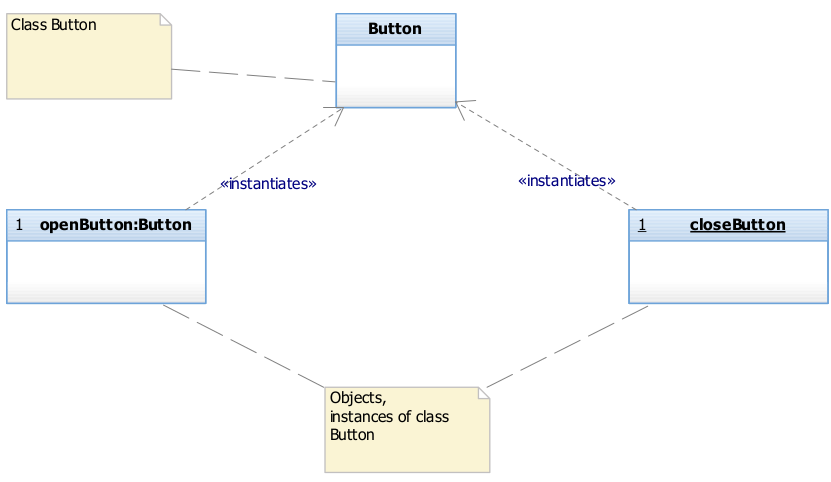
\includegraphics[width=0.49\textwidth]{images/UML/class_objects.png}
\end{paracol}

\subsubsection{Structure}
\begin{paracol}{2}
    Attributes define the structure of objects
    \begin{itemize}
        \item Attributes define properties of objects, which obtain and change their values during the lifetime of an object
        \item Attributes are also called member variables or properties
    \end{itemize}
    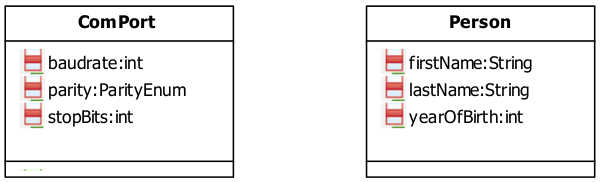
\includegraphics[width=0.49\textwidth]{images/UML/class_attributes.png}

    \switchcolumn

    Interfaces describe how objects can communicate with each other
    \begin{itemize}
        \item Objects communicate via operation-calls or asynchronous messages, e.g. event messages
        \item Events are triggers for state-machines
    \end{itemize}
    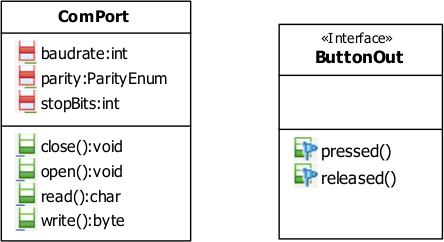
\includegraphics[width=0.39\textwidth]{images/UML/class_interfaces.png}
\end{paracol}

\subsubsection{Implementation}
Implementation describes the realisation of reactions to either operation-calls or events
\begin{itemize}
    \item The implementation of operations is defined in action-language (C, C++, UML-AL, ...)
    \item Reactions to events are defined in state-machines
\end{itemize}

\begin{paracol}{2}
    \subsubsection{State-Machine}
    \begin{itemize}
        \item Describes how objects of a specific class react to events
        \item Reaction depends on current state
        \item UML state-diagrams can be assigned to a UML class
        \item UML state-diagrams are used to describe state-machines for objects
    \end{itemize}
    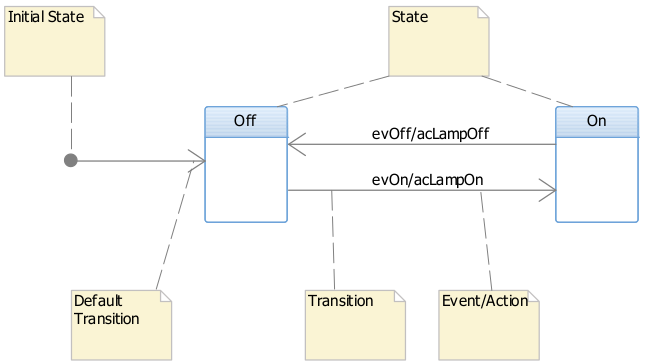
\includegraphics[width=0.49\textwidth]{images/UML/class_statemachine.png}

    \switchcolumn

    \subsubsection{Ports}
    \begin{itemize}
        \item Ports offer an additional possibility to define an interface
        \item A port consists of a provided (in) and/or a required (out) interface
        \item A port has a name, unique within its owning class
    \end{itemize}
    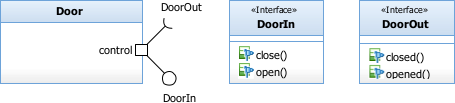
\includegraphics[width=0.49\textwidth]{images/UML/class_ports.png}
\end{paracol}

\subsubsection{Class Relationsships}
\begin{table}[h]
    \begin{tabularx}{\textwidth}{|l|X|X|}\hline
        Composition    & \raisebox{-.5\height}{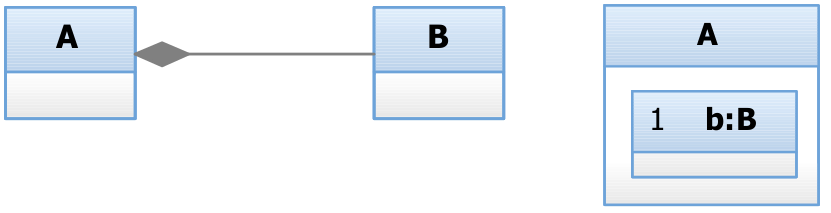
\includegraphics[width=0.3\textwidth]{images/UML/class_composition.png}}   & Instances of A contain instances of B. Some instances of B are part of an instance of A \\\hline
        Association    & \raisebox{-.5\height}{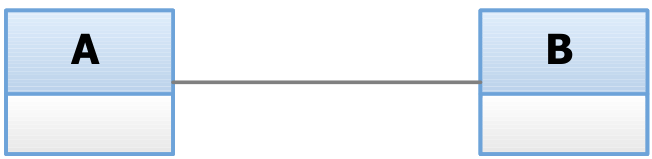
\includegraphics[width=0.185\textwidth]{images/UML/class_association.png}} & Instances of A are in some way releated to instances of B                               \\\hline
        Aggregation    & \raisebox{-.5\height}{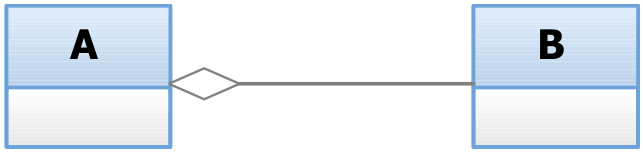
\includegraphics[width=0.185\textwidth]{images/UML/class_aggregation.png}} & A \glqq{}whole-part\grqq{} association                                                  \\\hline
        Generalization & \raisebox{-.5\height}{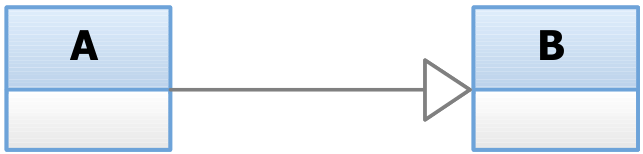
\includegraphics[width=0.185\textwidth]{images/UML/class_inheritance.png}} & A inherits structure and behaviour of B                                                 \\\hline
        Realization    & \raisebox{-.5\height}{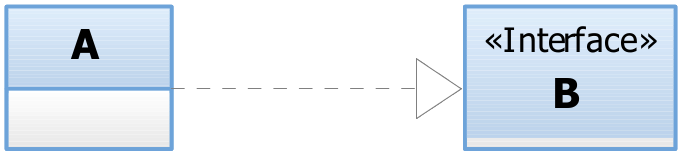
\includegraphics[width=0.185\textwidth]{images/UML/class_realization.png}} & A realises, i.e. implements the \glqq Interface\grqq{} B                                \\\hline
    \end{tabularx}
\end{table}

\paragraph{Cardinalities}
The cardinalities of a relationship describe how many objects are involved on each end of the relationship
% \begin{table}[h]
\begin{tabular}{ll}\hline
    Cardinality & Meaning   \\\hline
    0,1         & 0 or 1    \\\hline
    1           & exactly 1 \\\hline
    1..*        & 1 or more \\\hline
    0..*        & 0 or more \\\hline
\end{tabular}
% \end{table}
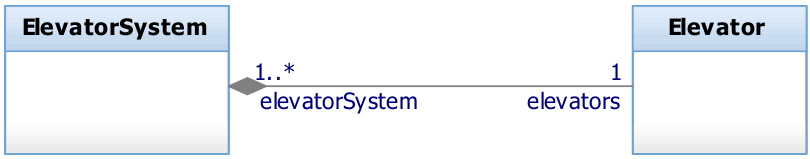
\includegraphics[width=0.5\textwidth]{images/UML/cardinality_example.png}

\paragraph{Navigability}\vspace{-12pt}
Directed: Elevator knows Door, but Door doesn't know Elevator
\raisebox{-.5\height}{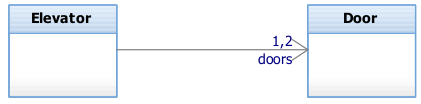
\includegraphics[width=0.3\textwidth]{images/UML/navi_directed.png}}

Bidirectional: Elevator knows ElevatorSystem and vice versa
\raisebox{-.5\height}{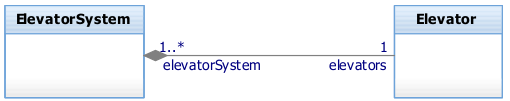
\includegraphics[width=0.37\textwidth]{images/UML/navi_bidirectional.png}}

\subsubsection{Polymorphism}
\begin{itemize}
    \item Many different implementations can realise (implement) the same interface (Figure)
    \item The caller (here Drawing) knows only the interface (Figure)
    \item For each instance the correct virtual operation draw, of the objects class, will be executed
\end{itemize}
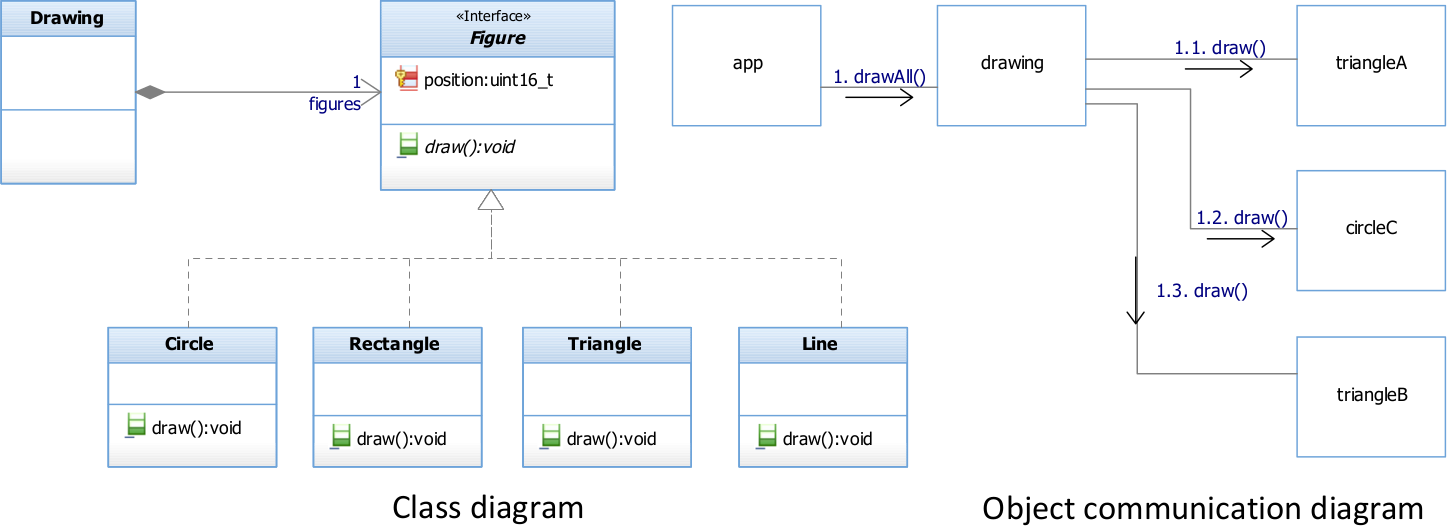
\includegraphics[width=1\textwidth]{images/UML/polymorphism.png}

\subsubsection{Structure Diagram}
\begin{itemize}
    \item Links are connections between objects or the ports
    \item Port links must connect compatible ports
    \item Object links are instances of associations between the corresponding classes
\end{itemize}
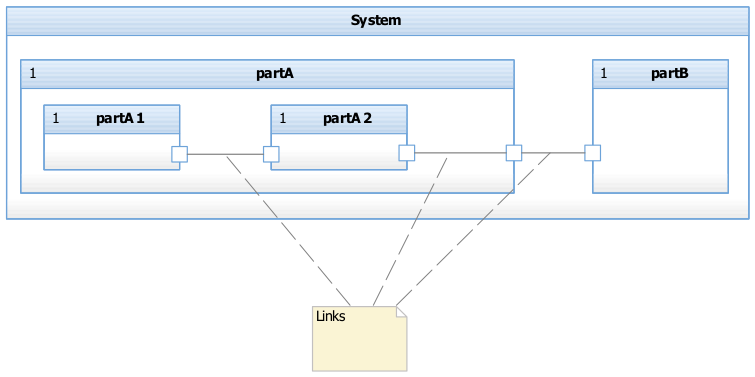
\includegraphics[width=0.8\textwidth]{images/UML/structure_diagram.png}


\subsection{State Diagram (Statechart)}
Technical processes may be visualized in state diagrams.

\begin{description}
    \item[Logical States] Dividing the set off all possible pyhsical states into a finite number of subsets
          \begin{itemize}
              \item so-called state classes
              \item a logical state corresponds to a state class
              \item by state of a technical process we mean its logical state
          \end{itemize}
    \item[Initial State] When the object is created, it enters the initial state and immediately takes the default transition
    \item[State Transition] State transitions in technical processes are triggered due to physical laws.
    \item[Event] Events are a consequence of a relevant state change of a technical process.
    \item[Attributes of Events] Events may hold attributes. Attributes may be any kind of additional information such as measureable quantities.
    \item[Time Events] Events based on time
    \item[Action] Actions are the means to control a technical process i.e. to have influence on it
          \begin{itemize}
              \item An action can indirectly cause a technical process to change its state
              \item The effect of an action depends on the current state of the technical-process
          \end{itemize}
    \item[Attributes of Actions] Actions may contain attributes
\end{description}
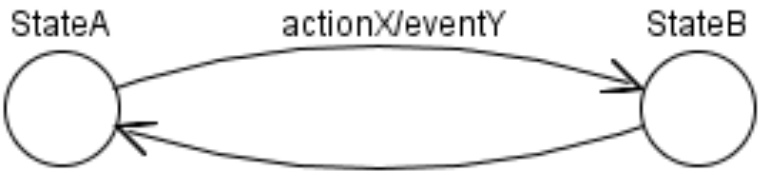
\includegraphics[width=0.35\textwidth]{images/UML/statechart.png}

\subsubsection{Advanced Features}
\begin{description}
    \item[Time-Events] Notation: after(100ms) (UML) or tm(timeUnits) (Rhapsody, where time units in ms)
    \item[Operation Calls in Actions] Operation calls can be part of an action.
          Operations are executed during transition.
          CIRO pulses are sent during state changes
    \item[Entry and Exit Actions] Actions executed on entry or exit of a state.
          Notation: Function call in body of state.
    \item[Internal Transitions]
\end{description}